%!TEX root = SSCR_project_main.tex
\chapter{Model Description}

\section{Class Diagram}
An initial UML class diagram was made, and later refined during the implementation. 
In Figure \ref{fig:SimpleClassDiagram} the final class diagram is shown.

\begin{figure}[H]
\centering
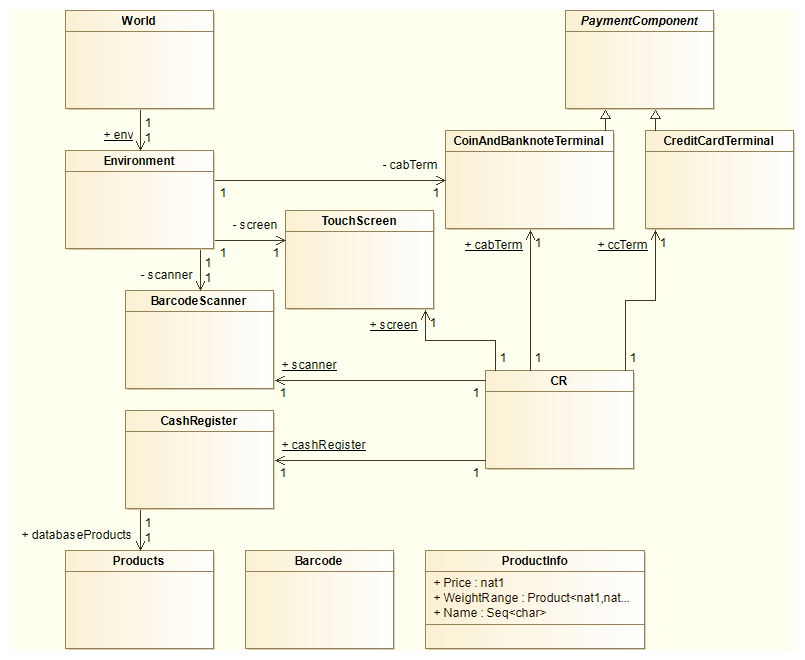
\includegraphics[width=0.8\linewidth]{SimpleClassDiagram}
\caption{Final class diagram.}
\label{fig:SimpleClassDiagram}
\end{figure}

The CR class is the 'system' class, which contains static references to all of the systems objects. 
The World and Environment classes are used to create stimuli to the system.

The CashRegister class contains most of the functionality. It is also this class that contains a database of all products and corresponding barcodes. 
It also contains a list of items in the 'shopping cart' and the accumulated price for the scanned products.

\newpage
\section{Class descriptions}

\subsection{World and Environment}
The World class is completely unnecessary, but is the entry for running the code.

The Environment class contains both a functional test in the run operation, and some traces. These are both explained further in chapter \ref{chp:Test}.

\subsection{CR}
The CR class is the system class, which contains static objects of all system classes. This is mainly to ease the implementation.
\begin{vdmpp}
class CR
 
instance variables
 public static cashRegister: CashRegister := new CashRegister(); 
 public static cabTerm: CoinAndBanknoteTerminal := new CoinAndBanknoteTerminal();
 public static ccTerm: CreditCardTerminal := new CreditCardTerminal();
 public static scanner: BarcodeScanner := new BarcodeScanner();
 public static screen: TouchScreen := new TouchScreen(); 
  
end CR
\end{vdmpp}

\subsection{TouchScreen}
The TouchScreen class represents the physical touch screen, but all GUI is abstracted away, and thus all operations are very simple, like the two examples show below.
\begin{vdmpp}
class TouchScreen

operations
 public StartPayment : () ==> ()
 StartPayment() ==
  CR`scanner.Enable(true);

 public PayCash : () ==> ()
 PayCash() ==
  CR`cashRegister.Pay(CR`cabTerm);
 \end{vdmpp}

\subsection{BarcodeScanner}
The BarcodeScanner class is similar to the TouchScreen class, but contains a single instance variable 'enable', to model that it could be turned on/off.


\subsection{PaymentComponent}
The PaymentComponent is a class with a single virtual Pay operation, with subclass responsibility. This means that all subclasses shall implement a corresponding pay function.
\begin{vdmpp}
public Pay : nat ==> bool
Pay(-) == is subclass responsibility;
\end{vdmpp}

\subsection{CoinAndBanknoteTerminal}
The CoinAndBanknoteTerminal is a subclass of the PaymentComponent, and therefore implements the Pay operation:
\begin{vdmpp}
class CoinAndBanknoteTerminal is subclass of PaymentComponent

instance variables
 balance : nat;

operations
 public Pay: nat ==> bool
  Pay(sum) ==
   let enough = sum < balance
      in
    if enough then
    (
     IO`print("Paying with cash: ");
     IO`print(sum);
     IO`print(" DKK\n");
     balance := balance - sum;
     RetreiveMoney();
     return true;
    ) else 
    (  
     IO`print("Insufficient funds.\n");
     return false;
    )
\end{vdmpp}

\subsection{CreditCardTerminal}
The CreditCardTerminal is also a subclass of PaymentComponent. Both internet access and pin code verification is abstracted away, since it is not of major importance in this project.

\begin{vdmpp}
 public Pay : nat ==> bool
 Pay(sum) ==
 (
  if(sum = 0) then
   return true; -- Nothing to pay
   
 --Emulate wrong pin, not enough money etc.
  if MATH`rand(100) < 10 then 
  (
   IO`print("Wrong PIN or insufficient funds.\n");
   return false;
  ) else 
  (  
   IO`print("Paying with credit card: ");
   IO`print(sum);
   IO`print(" DKK\n");
   return true;
  )
 );	
\end{vdmpp}

\newpage
\subsection{CashRegister}
The CashRegister class contains the main functionality in the system, and also the most interesting vdmpp syntax.

\subsubsection{Types and records}
The class contains three types definitions, including a map type and a record type:
\begin{vdmpp}
class CashRegister

types
 public Products = map Barcode to ProductInfo;
 public ProductInfo::  Price : nat1
            WeightRange : nat1 * nat1 --Not used yet
            Name : seq of char;
 public Barcode = nat1;
\end{vdmpp}

\subsubsection{Values and comprehensions}
Values are constant declarations, which are used here to populate the instance variable 'databaseProducts', which models a database of products. Both sequence and map comprehensions are used to generate these values.
\begin{vdmpp}
values
 prices : seq of nat1 = [ price | price in set {1,...,100} & price mod 10 = 0];
 weigths : seq of (nat1*nat1) = [ mk_(10*x, 20*x) | x in set elems prices];
 names : seq of (seq of char) = ["Bread","Milk","Honey","Ham","Touthpaste","Toilet paper","Beer",
 																"Pasta","Veal Beef","Ketchup"];
 
 public products : CashRegister`Products = {code |-> mk_CashRegister`ProductInfo(prices(code),
 																					weigths(code),names(code)) | code in set {1,...,10}}; 
\end{vdmpp}

\subsubsection{Invariants and expressions}
A few invariants are added to some of the instance variables. For the databaseProducts variable, it is to ensure that the database is not empty, and that all products have a name.
The invariant on the totalPrice is to ensure that the variable and the total price of all the products in the basket/shopping cart is equal.
\begin{vdmpp}
instance variables
 public databaseProducts: Products;
  inv databaseProducts <> {|->} and 
   forall x in set rng databaseProducts &
    x.Name <> "";
   
 basketProducts: seq of ProductInfo;
 totalPrice : nat;
  inv totalPrice = TotalPrice(basketProducts); 
\end{vdmpp}

\newpage
\subsubsection{Recursive functions}
In order to calculate the total price of all the products in the baskets, a recursive function is used. This is an easy way to iterate through a sequence and extract data from each element.
\begin{vdmpp}
functions
 TotalPrice : seq of ProductInfo -> nat
 TotalPrice(prods) == 
  if (len prods = 0) then
   0
  else
   (hd prods).Price + TotalPrice(tl prods)
  measure CardPrice;
  
 CardPrice : seq of ProductInfo -> nat
 CardPrice(prods) ==
  len prods; 
  
\end{vdmpp}

\subsubsection{Preconditions and atomic statement}
In the following the precondition is used on basketProducts. This ensures that the let expression does not throw a runtime error.
The atomic statement section is used, to ensure that the invariant on totalPrice is not broken, when updating the basketProducts. 
\begin{vdmpp}
 public AddMultiple : nat1 ==> ()
 AddMultiple(number) == 
  let prod = basketProducts(len basketProducts) 
   in  
    atomic
    (
      basketProducts := basketProducts ^ [prod|x in set {1,...,number-1}]
      totalPrice := totalPrice + prod.Price*(number-1);
    )
  pre len basketProducts <> 0;
\end{vdmpp}

\subsubsection{Benefits of inheritance}
One of the benefits with the inheritance from PaymentComponent to CoinAndBanknoteTerminal and CreditCardTerminal is, that the Pay operation in the CashRegister does not have to differentiate between the two payment methods, as seen in the following:
\begin{vdmpp}
 public Pay: (PaymentComponent) ==> ()
 Pay(component) ==
  (
   if component.Pay(totalPrice) then
   (
    IO`print("\nPayment receipt:\n");
    PrintReceipt(basketProducts);
    EmptyBasket();
    CR`scanner.Enable(false);
   )
  );
\end{vdmpp}


\subsubsection{Various operations}
The AddProduct operation contains various different vdmpp semantics, such as map and record application, sequence concatenation, etc.
The PrintReceipt operation is recursive, and displays a list of purchased groceries, as specified in requirement R.5.
\begin{vdmpp}
 public AddProduct: Barcode ==> ()
 AddProduct(bar) ==
  (
   if bar in set dom databaseProducts then
   (
    atomic
    (
     basketProducts := basketProducts ^ [databaseProducts(bar)];
     totalPrice := totalPrice + databaseProducts(bar).Price;
    );
   )
   else 
   (
    IO`print("Barcode is not valid\n");
   )
  );

 PrintReceipt: seq of ProductInfo ==> ()
 PrintReceipt(prods) ==
  if (len prods = 0) then
   return
  else
   let prod = hd prods
    in 
    (
     IO`print(prod.Name);
     IO`print(" : ");
     IO`print(prod.Price);
     IO`print(" DKK\n");
     PrintReceipt(tl prods);
    )
\end{vdmpp}